\subsection{新興技術のテストと新興技術によるテスト}
新興技術は、テスト対象として新しい課題を生む一方で、テスト活動を支援する手段にもなる。この章では、「新興技術をテストする」と「新興技術を使ってテストする」を分けて理解する。

\par\smallskip
\begin{center}
\centering
\IfFileExists{assets/generated_figures/ch05/fig-ch05-14.png}{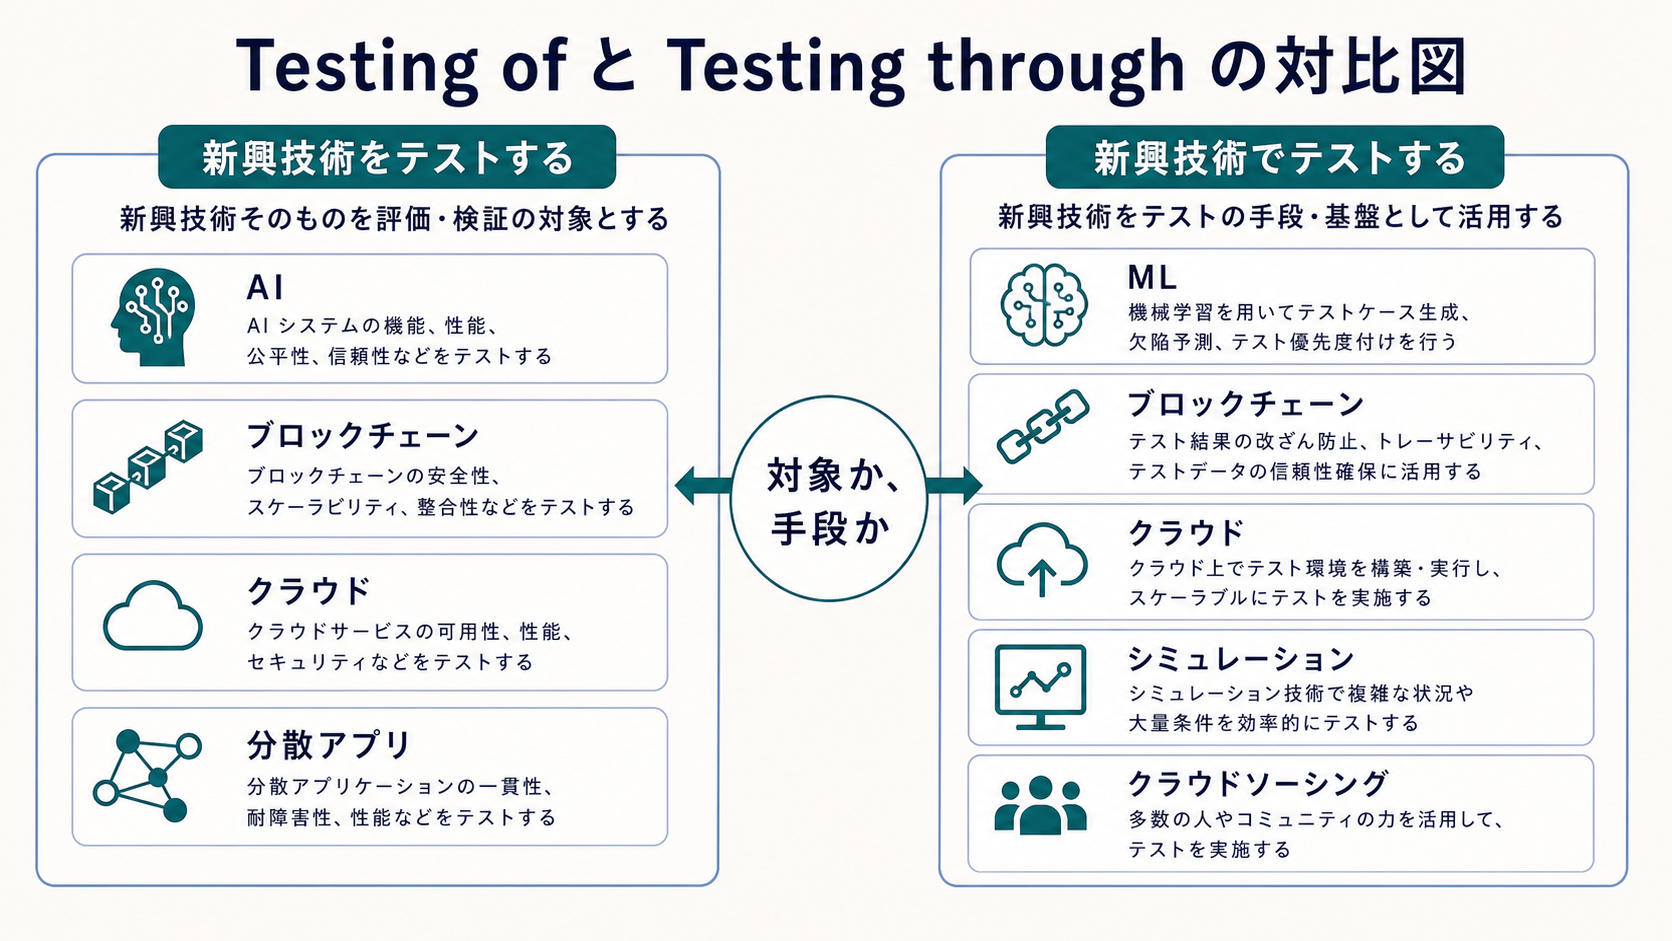
\includegraphics[width=0.96\linewidth]{assets/generated_figures/ch05/fig-ch05-14.png}}{\fbox{\parbox[c][48mm][c]{0.9\linewidth}{\centering 画像生成待ち\\Testing of と Testing through の対比図}}}
\par\smallskip
\refstepcounter{figure}\label{fig:ch05-14}図 \thefigure: Testing of と Testing through の対比図
\end{center}
図 \thefigure は、Testing of と Testing through の対比図を視覚的に整理したものである。
\par\smallskip

\subsubsection{新興技術をテストする}
AI、機械学習、深層学習を使ったシステムでは、非決定性、データ依存性、オラクル問題が大きな課題になる。欠陥は、学習データ、学習プログラム、モデル、フレームワーク、推論環境のどこにでもあり得る。オフラインでは交差検証などでモデルを評価し、配備後はオンラインテストで利用者行動との相互作用を評価する。

ブロックチェーンでは、スマートコントラクトや関連アプリケーションに対して、ストレステスト、侵入テスト、性質テストが使われる。公開型か私有型か、他アプリケーションとの接続、トランザクション性能、セキュリティなどを考慮する。

クラウドでは、クラウド上に配備されたアプリケーションやインフラの機能・非機能品質を確認する。性能、拡張性、弾力性、セキュリティ、互換性、相互運用性が重要である。分散・並行アプリケーションでは、複数 OS、ブラウザ、ハードウェア、利用者、依存関係、継続的配備がテストを複雑にする。

\subsubsection{新興技術を使ってテストする}
\term{機械学習}{Machine Learning}は、テストケース設計、オラクル問題、テスト評価、優先順位付け、ミューテーションテスト自動化、欠陥分類、トリアージに使われる。大量データから傾向を抽出し、保守労力を減らす可能性がある。

ブロックチェーンは、分散した関係者が信頼できる形でテスト活動を調整する手段になり得る。改ざん耐性、監査可能性、分散データ管理、要求順守の自動確認に役立つ可能性がある。クラウドは、大規模シミュレーションや弾力的資源を必要とするテスト環境として利用できる。

シミュレーションは、危険な状況、災害、復旧、特定振る舞いを評価するための重要な手段である。自動車や組込み領域では、実信号を SUT に与えながら現実を模擬するハードウェアインザループテストが使われる。クラウドソーシングテストは、多様な利用者、場所、端末、条件での検出力を得るために使われるが、社内検証の代替ではなく補完である。
